%
% $Id: $
%
%
% Compilar a .pdf con LaTeX (pdflatex)
% Es necesario instalar Beamer (paquete latex-beamer en Debian)
%

%
% Gr�ficos:
% Los gr�ficos pueden suministrarse en PNG, JPG, TIF, PDF, MPS
% Los EPS deben convertirse a PDF (usar epstopdf)
%

\documentclass{beamer}
\usetheme{Warsaw}
%\usebackgroundtemplate{
\includegraphics[width=\paperwidth]{format/libresoft-bg.png}}
%\usepackage[spanish]{babel}
\usepackage[latin1]{inputenc}
\usepackage{graphics}
\usepackage{amssymb} % Simbolos matematicos
\usepackage{url}

%\definecolor{libresoftgreen}{RGB}{162,190,43}
%\definecolor{libresoftblue}{RGB}{0,98,143}

%\setbeamercolor{titlelike}{bg=libresoftgreen}

%% Metadatos del PDF.
\hypersetup{
  pdftitle={ Dr. Scratch, an�lisis de proyectos Scratch para medir el desarrollo del Pensamiento Computacional y mejorar las habilidades de programaci�n},
  pdfauthor={Jes�s Moreno Le�n, Gregorio Robles},
  pdfcreator={GSyC/LibreSoft \\ Universidad Rey Juan Carlos},
  pdfproducer=PDFLaTeX,
  pdfsubject={Learning to code with Scratch. Automatic assesment.},
}
%%

\begin{document}

\title{Dr. Scratch}
\subtitle{An�lisis de proyectos Scratch para medir el desarrollo del Pensamiento Computacional y mejorar las habilidades de programaci�n}
\institute{jesus.moreno@programamos.es, grex@gsyc.urjc.es \\
GSyC/Libresoft, Universidad Rey Juan Carlos}
\author{Jes�s Moreno Le�n, Gregorio Robles}
\date{Seminario eMadrid, Fuenlabrada, 17 de abril de 2015}

\frame{
\maketitle
\begin{center}

\includegraphics[width=2cm]{format/libresoft-logo}
\hspace{0.5cm}

\includegraphics[width=5cm]{format/gsyc-urjc}
\vspace{0.5cm}

\includegraphics[width=3cm]{format/emadrid.png}
\end{center}
}


% Si el titulo o el autor se quieren acortar para los pies de p�gina
% se pueden redefinir aqu�:
%\title{Titulo corto}
%\author{Autores abreviado}

%% LICENCIA DE REDISTRIBUCION DE LAS TRANSPAS
\frame{
~
\vspace{3cm}

\begin{flushright}

\includegraphics[width=2.2cm]{figs/by-sa}

{\tiny
(cc) 2015 Gregorio Robles and Jes�s Moreno Le�n\\
  Some rights reserved. This work licensed under Creative Commons \\
  Attribution-ShareAlike License. To view a copy of full license, see \\
  http://creativecommons.org/licenses/by-sa/3.0/ or write to \\
  Creative Commons, 559 Nathan Abbott Way, Stanford, \\
  California 94305, USA. \\
\ \\
Some of the figures have been taken from the Internet \\
Source, and author and licence if known, is specified. \\
For those images, \emph{fair use} applies.
}
\end{flushright}
}
%%

\section{Seminario eMadrid sobre Pensamiento Computacional}


%--------------------------------------------------------
\usebackgroundtemplate{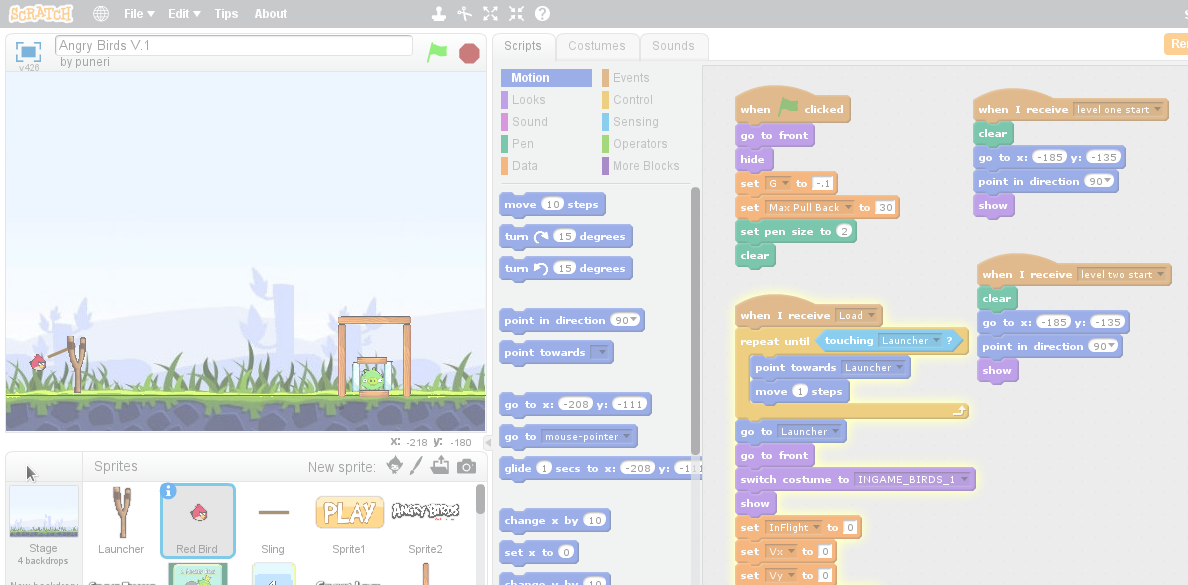
\includegraphics[width=18cm]{figs/AngryBirds.png}}

\begin{frame}
\frametitle{�Qu� es Scratch?}

\begin{center}
\Huge {\bf Programaci�n para todos. Programar para aprender.}
\end{center}

\end{frame}

\usebackgroundtemplate{}
%--------------------------------------------------------
%\usebackgroundtemplate{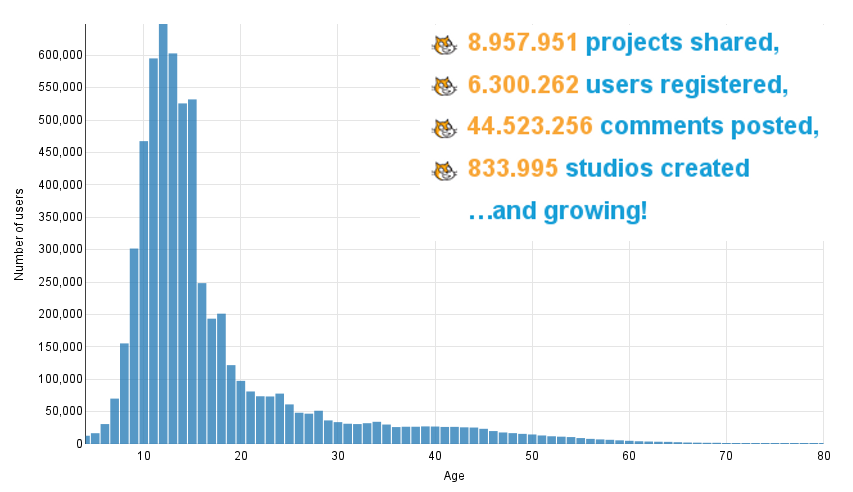
\includegraphics[width=18cm]{figs/stats.png}}

\begin{frame}
\frametitle{�Qui�n usa Scratch?}
\begin{figure}[t!]
\begin{center}
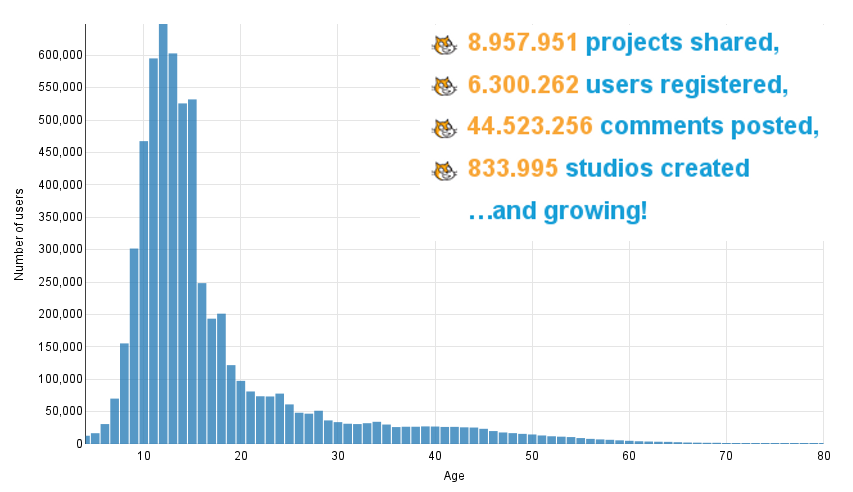
\includegraphics[width=10cm, height=6cm]{figs/stats.png}
\end{center}
\label{fig:naming}
\end{figure}
\begin{center}
scratch.mit.edu/statistics
\end{center}
\end{frame}

%--------------------------------------------------------
%\usebackgroundtemplate{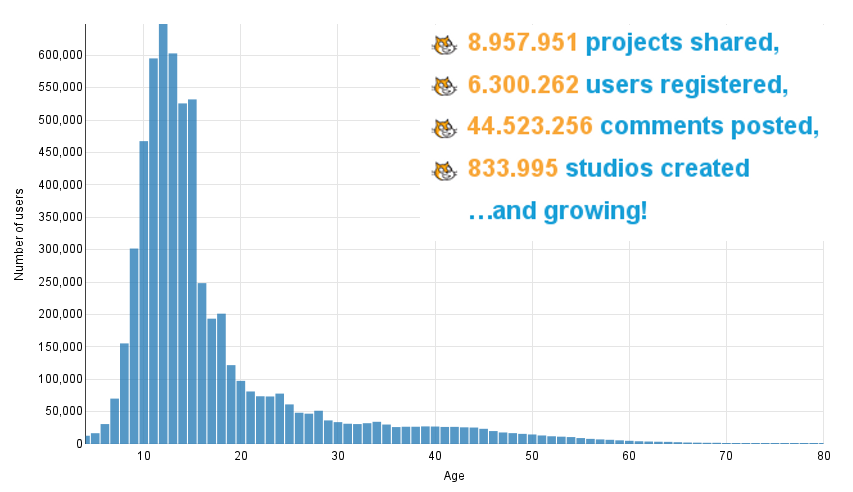
\includegraphics[width=18cm]{figs/stats.png}}

\begin{frame}
\frametitle{�Por qu� una herramienta como Dr. Scratch?}
\begin{figure}[t!]
\begin{center}

\includegraphics[width=5cm, height=6cm]{figs/cara.png}
\end{center}
\label{fig:naming}
\end{figure}
\begin{center}
Disfrutando de corregir proyectos Scratch
\end{center}
\end{frame}

%--------------------------------------------------------
%\usebackgroundtemplate{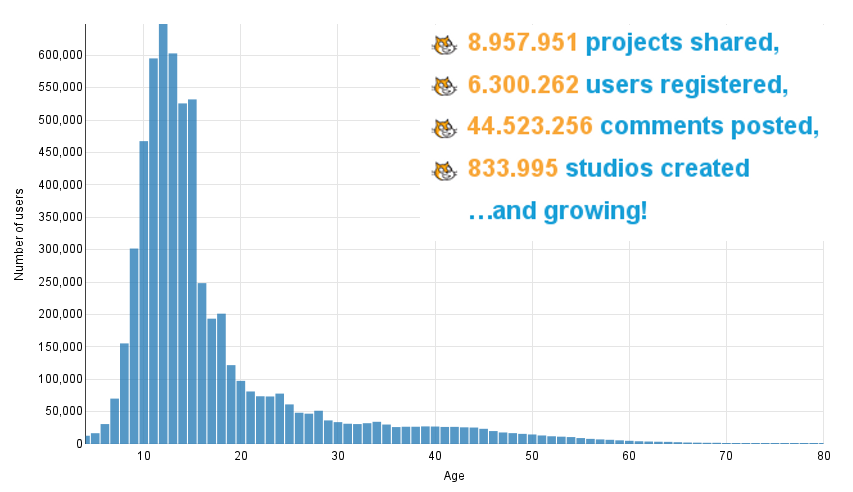
\includegraphics[width=18cm]{figs/stats.png}}

\begin{frame}
\frametitle{Revisi�n de la literatura}
\begin{columns}[T]
    \begin{column}{1\textwidth}
     \begin{block}{Evaluaci�n de proyectos Scratch}
\begin{itemize}
  \item Varios marcos para realizar an�lisis manuales.
  \item \texttt{Scrape}: Analizador del portfolio de un usuario para visualizar los bloques utilizados.
  \item \texttt{Hairball}: Analizador est�tico de proyectos Scratch inspirado en \texttt{lint} para detectar errores de programaci�n.
\end{itemize}
    \end{block}
    \end{column}
  \end{columns}
\end{frame}

%--------------------------------------------------------
\begin{frame}
\frametitle{Malos h�bitos de programaci�n con Scratch (I)}

\begin{figure}[t!]
\begin{center}
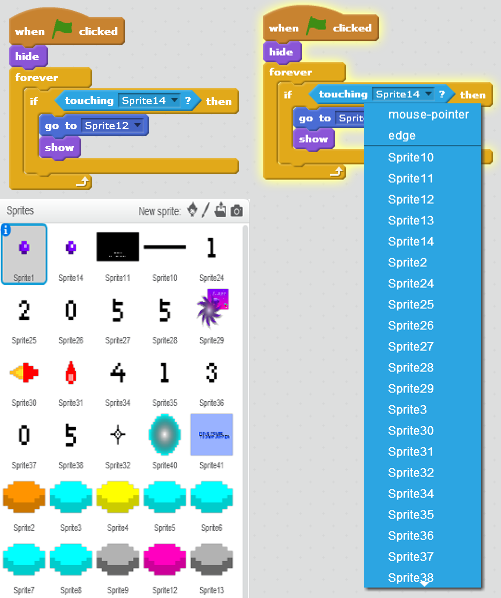
\includegraphics[width=7cm, height=6cm]{figs/SpriteNaming.png}
\end{center}
\label{fig:naming}
\end{figure}

\begin{center}
Nombres de personajes \emph{incorrectos}/por defecto
\end{center}
\end{frame}

%--------------------------------------------------------
\begin{frame}
\frametitle{Malos h�bitos de programaci�n con Scratch (y II)}

  \begin{columns}[T]
    \begin{column}{0.5\textwidth}
 
     \begin{block}{Ejemplo de c�digo repetido}
\begin{figure}[t!]
\begin{center}
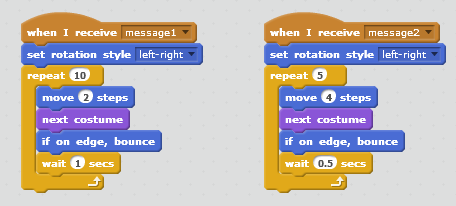
\includegraphics[width=5.4cm,height=2.5cm]{figs/CodeRepetition1.png}
\end{center}
\label{fig:repetition1}
\end{figure}
     \end{block}
    \end{column}
    \begin{column}{0.5\textwidth}
     \begin{block}{Evitar la repetici�n de c�digo}
\begin{figure}[t!]
\begin{center}
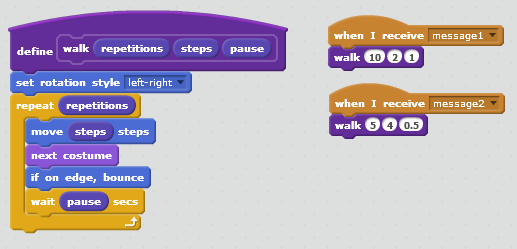
\includegraphics[width=5.4cm,height=2.5cm]{figs/CodeRepetition2.png}
\end{center}
Deben definirse bloques para evitar la repetici�n de c�digo
\label{fig:repetition2}
\end{figure}
     \end{block}

    \end{column}
  \end{columns}

\end{frame}

%--------------------------------------------------------
%--------------------------------------------------------
\usebackgroundtemplate{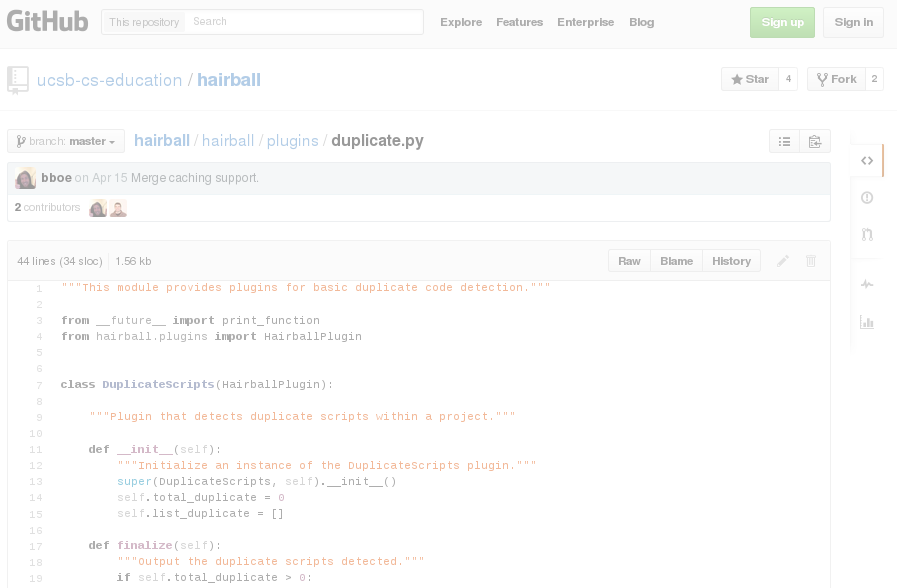
\includegraphics[width=13cm,height=9.2cm]{figs/plugins.png}}
% background: http://25.media.tumblr.com/b83aa72682992ab34b8ce7e61c0cb7f9/tumblr_menxc7qcq61ryin08o1_r1_1280.jpg
\begin{frame}
\frametitle{Desarrollo de plug-ins para \texttt{Hairball}}

  \begin{columns}[T]
    \begin{column}{0.8\textwidth}
     \begin{block}{\vspace{0.1cm}\center{Desarrollamos dos plug-ins para \texttt{Hairball} para detectar autom�ticamente estos malos h�bitos de programaci�n}\vspace{0.1cm}}
\vspace{0.3cm}
\begin{enumerate}
  \item convention.SpriteNaming
\vspace{0.15cm}
  \item duplicate.DuplicateScripts
\end{enumerate}
\vspace{0.4cm}
    \end{block}
    \end{column}
  \end{columns}

\end{frame}

\usebackgroundtemplate{}

%--------------------------------------------------------
%\usebackgroundtemplate{\includegraphics[width=13cm]{figs/iceberg.jpg}}
% background: http://www.wim-network.org/wp-content/uploads/2012/04/iceberg.jpg

\begin{frame}
\frametitle{An�lisis del repositorio de proyectos Scratch}

\begin{table}
\begin{center}
  \begin{tabular}{ | l | c | c | c |}
   \hline
              & Nombres por def. & Prog. Duplicados & Bloques propios \\ \hline\hline
    Proyectos & 79 & 62 & 17 \\ \hline
    Media & 5.94 & 7.23 & 1.11 \\ \hline
    Mediana & 3 & 2 & 0 \\ \hline
    M�ximo & 67 & 71 & 25 \\
    \hline    
  \end{tabular}
\end{center}
\caption{An�lisis de 100 proyectos Scratch descargados aleatoriamente}
\label{table:results}
\end{table}
\end{frame}

%--------------------------------------------------------
\usebackgroundtemplate{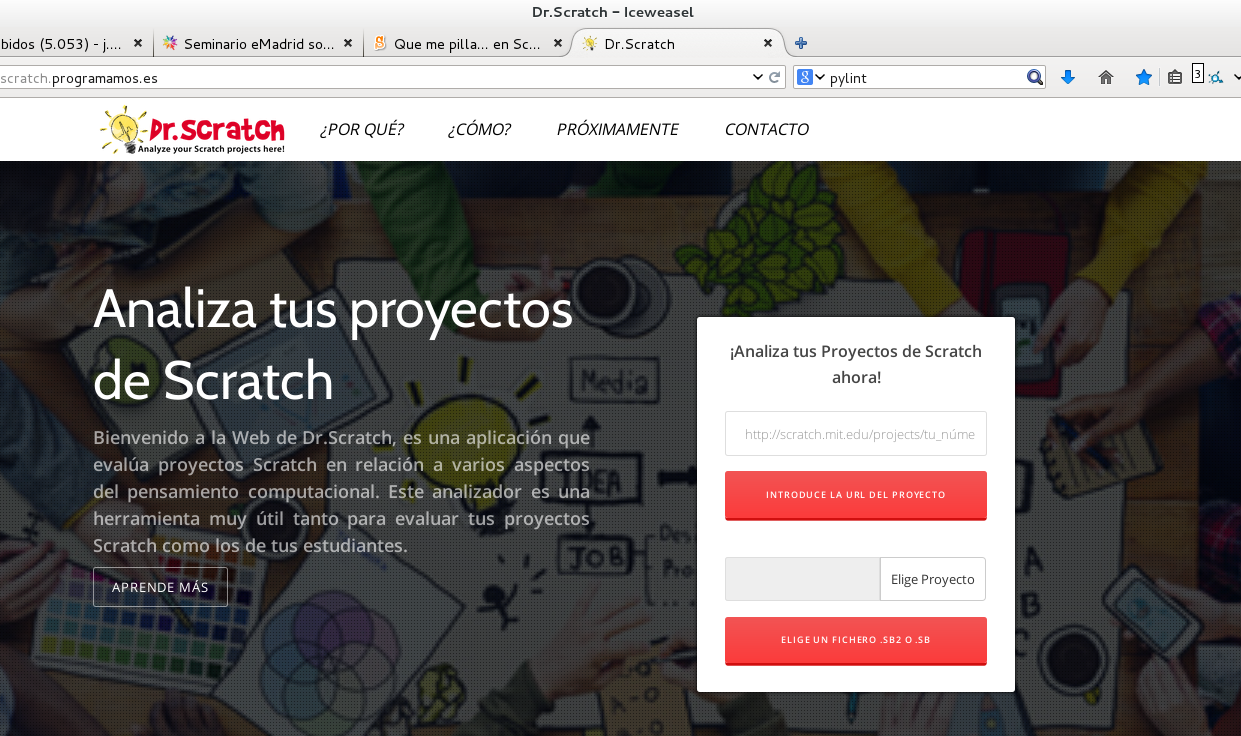
\includegraphics[width=13cm, height=9cm]{figs/drscratch.png}}
% background: http://www.wim-network.org/wp-content/uploads/2012/04/iceberg.jpg

\begin{frame}
\frametitle{Dr. Scratch}

\end{frame}

\usebackgroundtemplate{}

%--------------------------------------------------------
%\usebackgroundtemplate{\includegraphics[width=13cm]{figs/iceberg.jpg}}
% background: http://www.wim-network.org/wp-content/uploads/2012/04/iceberg.jpg

\begin{frame}
\frametitle{Dr. Scratch: an�lisis del Pensamiento Computacional}
\begin{table}[t]\tiny 
\centering
%\begin{tabular}{p{2.5cm}p{2.7cm}p{3cm}p{4cm}}
\begin{tabular}{|p{2cm}|p{2cm}|p{2cm}|p{2cm}|}
%\toprule
\hline
Componente PC & B�sico & En desarrollo & Avanzado\\ %\midrule 
\hline
\hline  
Representaci�n de la informaci�n & modifiers of sprites properties &
operations on vars & operations on lists  \\
\hline
Pensamiento L�givo & if & if else & logic operations \\ 
\hline
Interactividad con el usuario & green flag & key pressed, sprite clicked, ask and wait,
mouse blocks & when \%s is \textgreater \%s, video, audio \\ 
\hline
Control de flujo & sequence of blocks & repeat, forever & repeat until \\ 
\hline
Abstracci�n & more than one script and more than one sprite & def block & when I start as clone\\
\hline
Paralelismo & Two scripts on green flag & Two scripts on key pressed, two scripts on sprite clicked on the same sprite & Two scripts on when I receive message, create clone, two scripts when \%s is \textgreater \%s, two scripts on when backdrop change to \\
\hline
Sincronizaci�n & wait & Broadcast, when I receive message, stop all, stop program, stop programs sprite & wait until, when backdrop change to, broadcast and wait \\ 
\hline
\end{tabular}
\caption{Nivel de desarrollo para cada componente del Pensamiento Computacional.}
\label{table:CTscore}
\end{table}

\end{frame}


%--------------------------------------------------------
%\usebackgroundtemplate{
\includegraphics[width=13cm]{figs/take-away.jpg}}
% background: http://2.bp.blogspot.com/-78Eh4TBpdtU/UPw7ULV73PI/AAAAAAAAHAE/6DQfvPNCo-Y/s1600/8723052-stylized-red-stamp-showing-the-term-take-away-all-on-white-background.jpg
\usebackgroundtemplate{
\includegraphics[width=13cm]{figs/future.png}}

\begin{frame}
\frametitle{Future Work}

\begin{enumerate}
  \item Extend the scope of the study developing new plug-ins
  \item Analyze dataset with 5 years of data from the Scratch website
  \item Dr. Scratch (alpha version): http://drscratch.programamos.es
\end{enumerate}
\vspace{\baselineskip}
\vspace{\baselineskip}
\hfill{\Tiny Background picture: Simon Cunningham }

\end{frame}

%--------------------------------------------------------
%\begin{frame}
%\frametitle{GSyC/LibreSoft}

%\begin{figure}[t!]
%\begin{center}
%\includegraphics[width=11cm]{figs/libresoft.jpg}
%\end{center}
%\label{fig:libresoft}
%\end{figure}

%\begin{center}
%The GSyC/LibreSoft research team at URJC (Madrid).
%\end{center}

%\end{frame}

%--------------------------------------------------------
%\begin{frame}
%\frametitle{Our work at GSyC/LibreSoft}

%\begin{figure}[t!]
%\begin{center}
%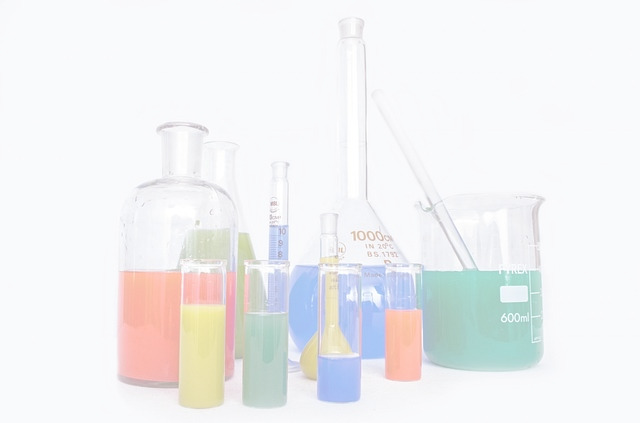
\includegraphics[width=2.5cm]{figs/research}
% http://www.memphis.edu/crow/images/research_2.jpg
%\hspace{0.1cm}
%\includegraphics[width=2.5cm]{figs/teaching}
% http://2.bp.blogspot.com/_uxgwfriLwSo/TOWDr8IjaLI/AAAAAAAABLM/d7H-G5jIq-c/s1600/teaching.gif
%\hspace{0.1cm}
%\includegraphics[width=2.5cm]{figs/development}
% http://www.vidadigitalradio.com/wp-content/uploads/2009/04/hackers_cartoons.jpg
%\hspace{0.1cm}
%\includegraphics[width=2.5cm]{figs/promotion}
% http://bloggeate.com/wp-content/uploads/2011/04/como-promocionar-tu-blog.jpg
%\end{center}
%\label{fig:whatwedo}
%\end{figure}

%\begin{center}
%GSyC/LibreSoft's tasks: research, teaching, development, promotion of free software.

%\end{center}
%\end{frame}

\usebackgroundtemplate{}

%--------------------------------------------------------
\frame{
\maketitle
\begin{center}

\includegraphics[width=2cm]{format/libresoft-logo}
\hspace{0.5cm}

\includegraphics[width=5cm]{format/gsyc-urjc}
\vspace{0.5cm}

\includegraphics[width=3cm]{format/emadrid.png}
\end{center}
}

\end{document}
